\documentclass[a4paper, 12pt]{article}

\usepackage{wrapfig}
\usepackage{graphicx}
\usepackage{mathtext}
\usepackage{amsmath}
\usepackage{siunitx}
\usepackage{multirow}
\usepackage{rotating}

\usepackage[T1,T2A]{fontenc}

\usepackage[russian]{babel}

\graphicspath{{pictures/}}

\title{\begin{center}Лабораторная работа №1.4.5\end{center}
Изучение колебаний струны}
\author{Гёлецян А.Г.}
\date{\today}

\begin{document}
    \pagenumbering{gobble}
    \maketitle
    \newpage
    \pagenumbering{arabic}

    \section{Ход работы}
    \begin{table}[h!]
        \begin{center}
        \begin{tabular}{|l|r|r|r|r|r|r|r|r|r|r|}
        \hline
        $m, г$ &   $F, н$ & $\nu_1, Гц$ & $\nu_2, Гц$ & $\nu_3, Гц$ & $\nu_4, Гц$ & $\nu_5, Гц$ & $\nu_6, Гц$ & $\nu_7, Гц$ & $\nu_8, Гц$ & $\nu_9, Гц$ \\\hline
        1095.5 &  10.75 &  137.0 &  278.3 &  413.8 &  560.7 &   694.1 &   844.0 &   975.9 &  1127.0 &  1263.8 \\\hline
        1577.3 &  15.48 &  164.3 &  330.0 &  495.5 &  661.0 &   827.6 &   994.4 &  1161.3 &  1329.0 &  1497.0 \\\hline
        2064.7 &  20.27 &  188.0 &  377.3 &  565.9 &  755.4 &   945.0 &  1135.2 &  1325.9 &  1518.0 &  1709.0 \\\hline
        2545.1 &  24.98 &  210.0 &  420.9 &  631.3 &  842.0 &  1053.6 &  1265.2 &  1477.0 &  1690.3 &  1903.7 \\\hline
        3027.5 &  29.72 &  228.0 &  457.0 &  685.0 &  914.0 &  1141.0 &  1370.0 &  1599.0 &  1828.0 &  2061.0 \\\hline

        \end{tabular}
         \caption{Измерения гармоник в зависимости от силы натяжения}
        \end{center}

    \end{table}

    \paragraph{}
    Ускорение свободного падения $g = (9.8155 \pm 0.0005)мс^{-2}$.
    Погрешнось измерения массы $\Delta m=0.1г$. Погрешность силы
    \[\varepsilon_F=\sqrt{{\left(\frac{\Delta g}{g}\right)}^2 +
    {\left(\frac{\Delta m}{m}\right)}^2}\approx10^{-4}\]
    Это на порядки меньше остальных погрешностей, поэтому учитывать его не будем.


    \[u = 2l\nu_1\]
    Где
    \[l = (50.0 \pm 0.1)см\]

    \paragraph{}
    Из графиков получаем.

    \begin{table}[h!]
        \begin{center}
        \begin{tabular}{|l|r|r|r|r|r|}
        \hline
        $F, Н$             & 10.75 & 15.48 & 20.27 & 24.98 & 29.72 \\\hline
        $\nu_1, Гц$        & 141.0 & 166.5 & 190.1 & 211.6 & 228.8 \\\hline
        $\Delta \nu_1, Гц$ &   1.1 &   0.3 &   0.4 &   0.4 &   0.4 \\\hline
        \end{tabular}
        \caption{Зависимость частоты первой гармоники от натяжения}
        \end{center}
    \end{table}
    Так как $2l=1м$ то числовые значения u в $мс^{-1}$ совподают с значениями $\nu_1$ в $Гц$.

    \paragraph{}
    Из графика $u^2(F)$ получаем
    \[\frac{1}{\rho}=(1730\pm40)м^3кг^{-1}\]
    \[\Delta \left(\frac{1}{\rho}\right) = \frac{\Delta \rho}{\rho^2}\]
    Подставляя чиссла получаем
    \[\rho = (578 \pm 13)\muг/м\]
    Что совпадает с реальным значением $\rho_l=568.4\muг/м$ в пределах погрешности.
    \newpage
    \begin{sidewaysfigure}
        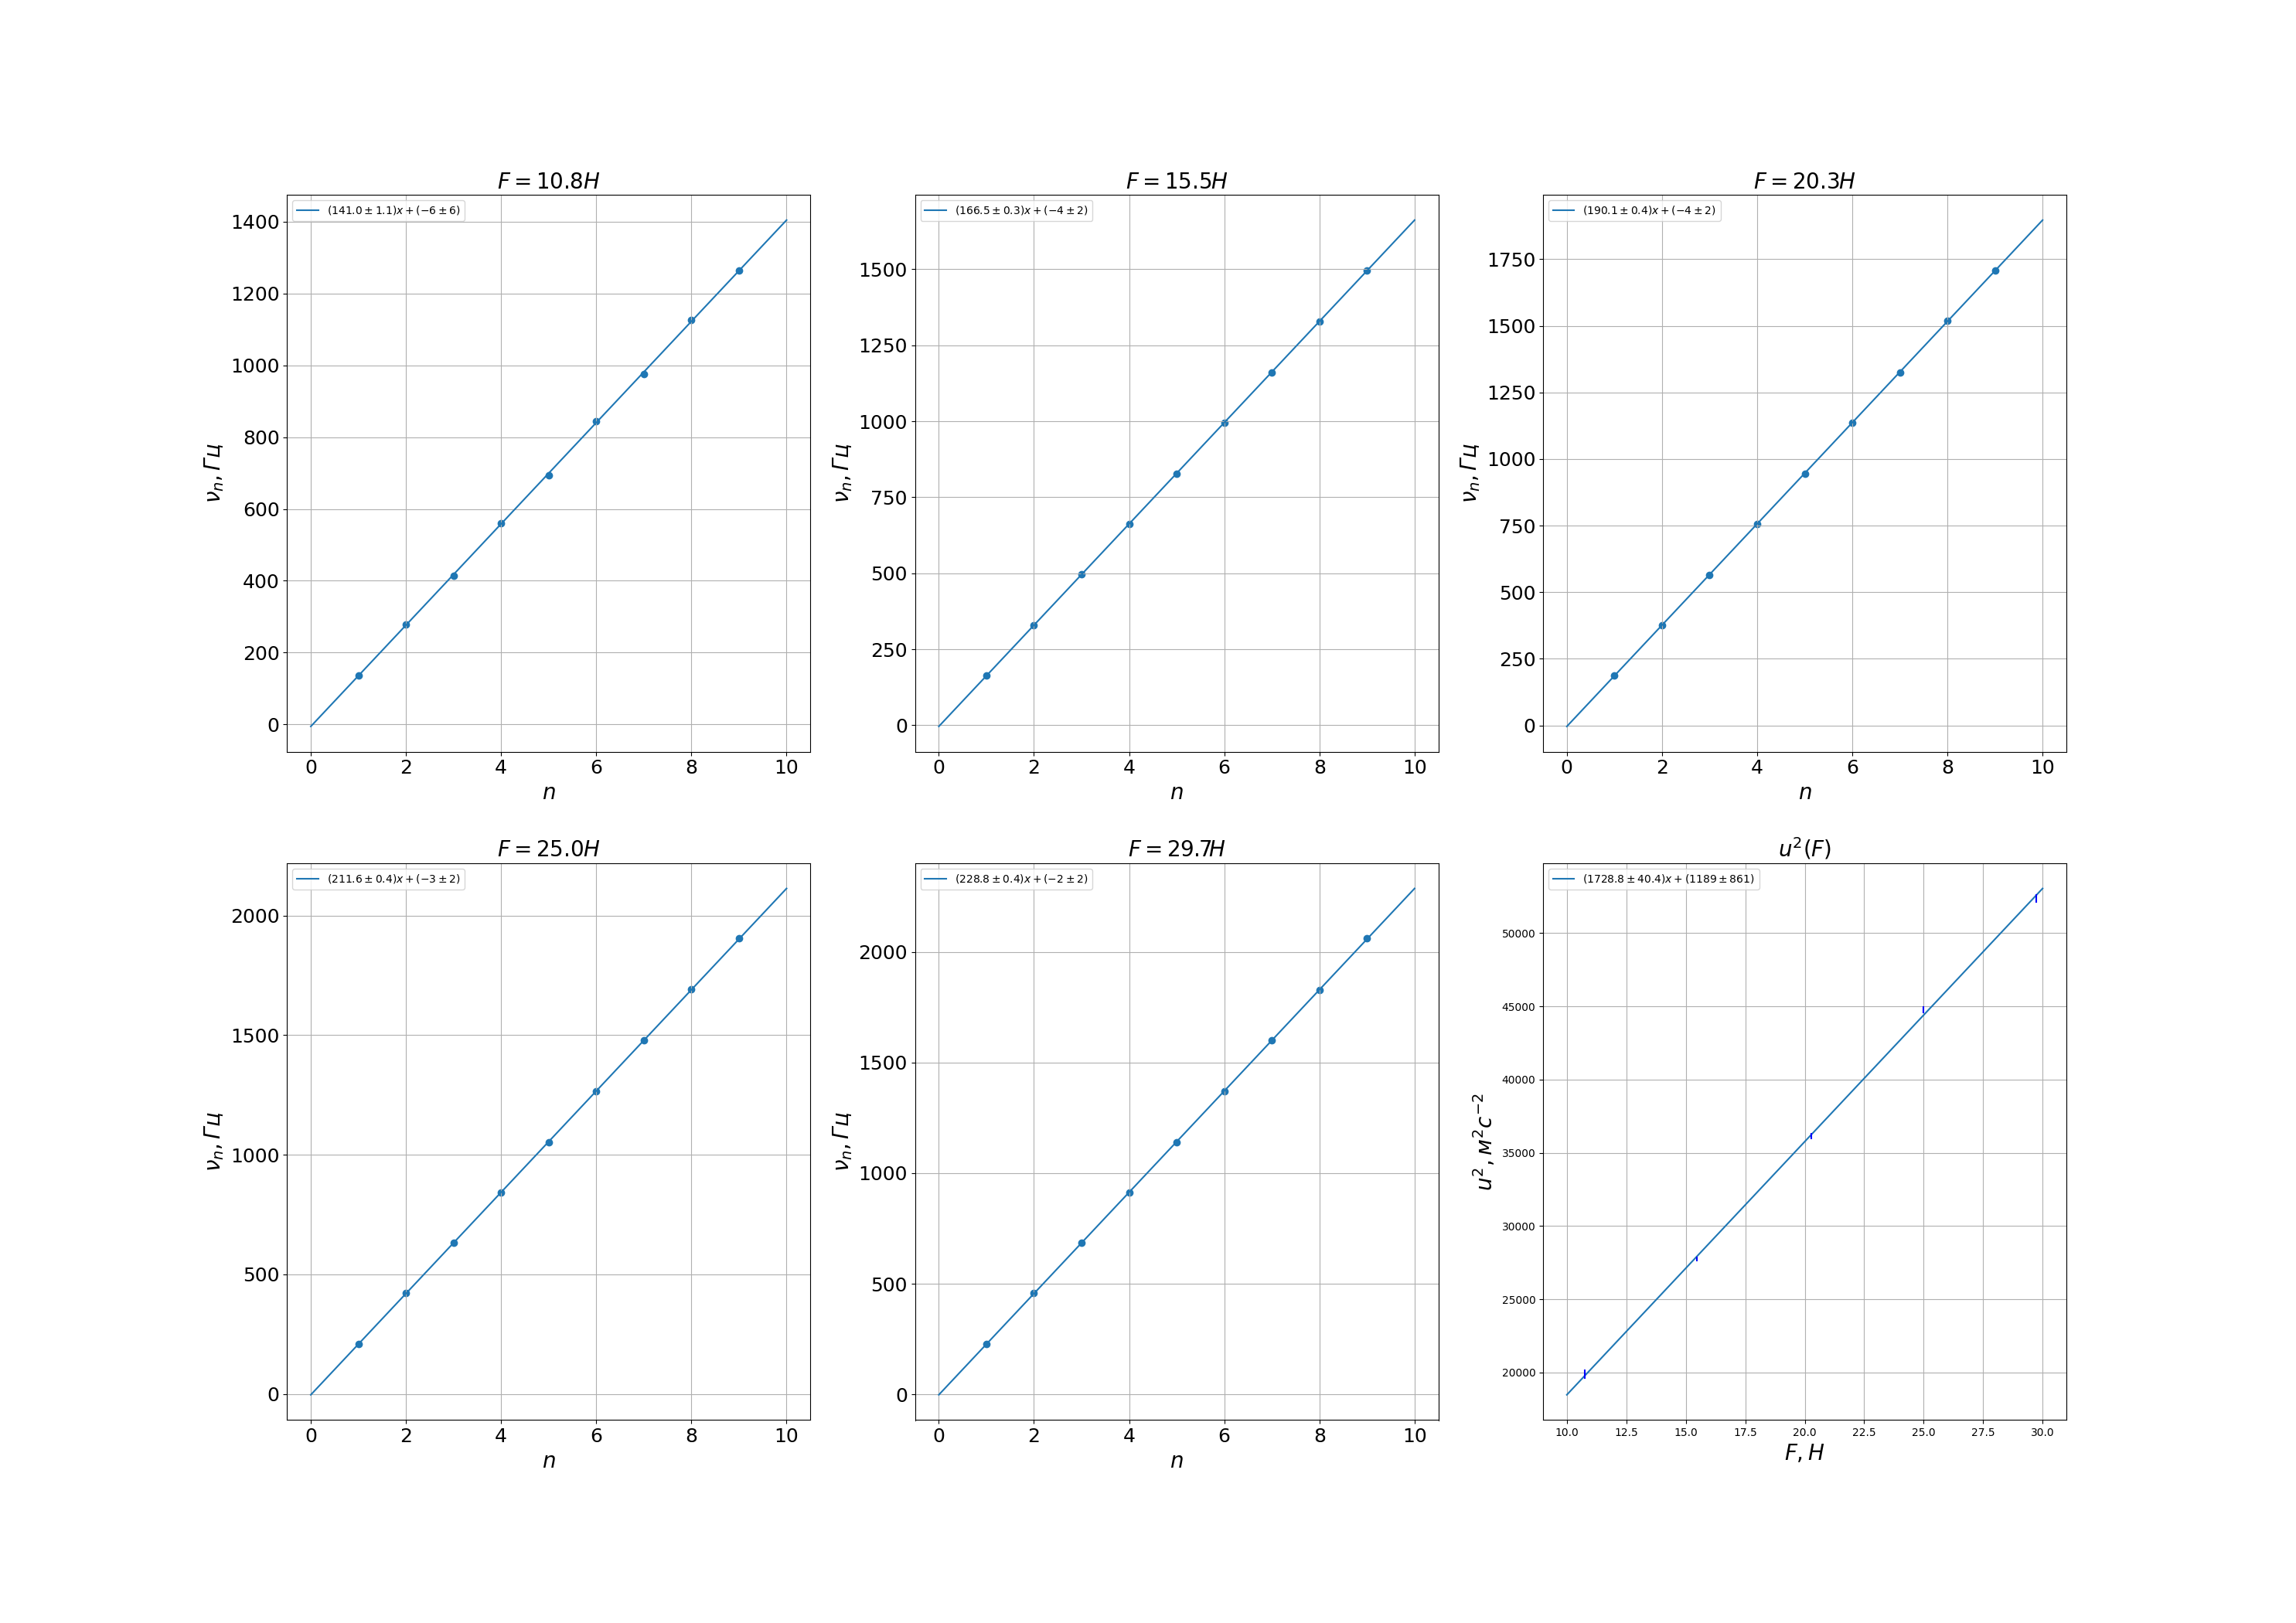
\includegraphics[width=1.2\textwidth]{plots.png}
        \caption{Графики}
    \end{sidewaysfigure}
\end{document}

